\chapter{Supplementary information}


\begin{table}[!h]
    \centering
    \caption{Highly variable genes on pooled data and subsampled data by condition}
    \begin{tabular}{llll}
    \hline
        \textbf{} & \textbf{Global} & \textbf{Colorectal carcinoma} & \textbf{Healthy samples} \\ \hline
        ASCT2 & ~ & ~ & ~ \\
        ATP5A & ~ & ~ & ~ \\
        CD11c & ~ & ~ & ~ \\
        CD14 & X & ~ & X \\
        CD3 & X & X & X \\
        CD31 & ~ & ~ & ~ \\
        CD36 & X & ~ & X \\
        CD39 & ~ & ~ & ~ \\
        CD4 & ~ & ~ & X \\
        CD45 & X & X & X \\
        CD57 & ~ & ~ & ~ \\
        CD68 & ~ & ~ & ~ \\
        CD8 & ~ & X & ~ \\
        CD98 & X & X & X \\
        CK & X & ~ & ~ \\
        CPT1A & ~ & ~ & ~ \\
        CS & ~ & ~ & ~ \\
        Ecad & ~ & ~ & ~ \\
        G6PD & X & X & X \\
        GLUT1 & ~ & ~ & ~ \\
        H3 & X & X & X \\
        HIF1A & X & X & X \\
        HK1 & X & ~ & X \\
        IDH2 & ~ & ~ & ~ \\
        Ki67 & X & X & X \\
        LDHA & ~ & ~ & X \\
        NRF2p & X & X & ~ \\
        NaKATPase & X & X & X \\
        PD1 & ~ & ~ & ~ \\
        PKM2 & X & ~ & X \\
        S6p & X & X & X \\
        SDHA & ~ & X & ~ \\
        SMA & ~ & X & ~ \\
        VDAC1 & X & X & ~ \\
        XBP1 & ~ & X & ~ \\
        vimentin & ~ & X & X \\[0.4cm]
        \multicolumn{4}{l}{\scriptsize X: Highly variable gene} \\
    \end{tabular}
    \label{tab:sup-hvargs}
\end{table}


\begin{table}[!h]
    \centering
    \caption{Moran I scores and their respective FDR corrected p-values under the assumption of normality applied to colorectal cancer sample "Point23" and healthy colon sample "Point49"}
    \begin{tabular}{ l p{3cm} p{3cm} p{3cm} p{3cm}}
    \hline
        \textbf{} & \textbf{Moran's I \newline cancer sample} & \textbf{p-val FDR-BJ cancer sample} & \textbf{Moran's I \newline healthy sample} & \textbf{p-val FDR-BH healthy sample} \\ \hline
        ASCT2 & 0.434129 & 0 & 0.198777 & 0 \\
        ATP5A & 0.258313 & 0 & 0.352868 & 0 \\
        CD11c & 0.764473 & 0 & 0.664476 & 0 \\
        CD14 & 0.451225 & 0 & 0.593698 & 0 \\
        CD3 & 0.46889 & 0 & 0.575716 & 0 \\
        CD31 & 0.378775 & 0 & 0.237861 & 0 \\
        CD36 & 0.487321 & 0 & 0.185019 & 0 \\
        CD39 & 0.552447 & 0 & 0.332658 & 0 \\
        CD4 & 0.601358 & 0 & 0.511698 & 0 \\
        CD45 & 0.781277 & 0 & 0.755632 & 0 \\
        CD57 & 0.0119118 & 0.240685 & 0.096923 & 5.7088e-11 \\
        CD68 & 0.390981 & 0 & 0.363916 & 0 \\
        CD8 & 0.303137 & 0 & 0.188665 & 0 \\
        CD98 & 0.586363 & 0 & 0.591238 & 0 \\
        CK & 0.861324 & 0 & 0.870824 & 0 \\
        CPT1A & 0.387363 & 0 & 0.439394 & 0 \\
        CS & 0.429202 & 0 & 0.446503 & 0 \\
        Ecad & 0.450744 & 0 & 0.617346 & 0 \\
        G6PD & 0.300406 & 0 & 0.120117 & 7.05318e-16 \\
        GLUT1 & 0.591208 & 0 & 0.557849 & 0 \\
        H3 & 0.418025 & 0 & 0.516858 & 0 \\
        HIF1A & 0.0297889 & 0.0451517 & 0.386171 & 0 \\
        HK1 & 0.616579 & 0 & 0.404228 & 0 \\
        IDH2 & 0.405139 & 0 & 0.300103 & 0 \\
        Ki67 & 0.145286 & 3.33067e-16 & 0.572123 & 0 \\
        LDHA & 0.715174 & 0 & 0.528124 & 0 \\
        NRF2p & 0.27139 & 0 & 0.254227 & 0 \\
        NaKATPase & 0.599137 & 0 & 0.704375 & 0 \\
        PD1 & 0.428382 & 0 & 0.400004 & 0 \\
        PKM2 & 0.670421 & 0 & 0.561082 & 0 \\
        S6p & 0.477971 & 0 & 0.510066 & 0 \\
        SDHA & 0.254028 & 0 & 0.320846 & 0 \\
        SMA & 0.419539 & 0 & 0.444856 & 0 \\
        VDAC1 & 0.323745 & 0 & 0.137777 & 0 \\
        XBP1 & 0.159283 & 0 & 0.0620587 & 1.69041e-05 \\
        vimentin & 0.507407 & 0 & 0. & ~ \\
    \end{tabular}
    \label{tab:sup-moran}
\end{table}


\begin{table}[!h]
    \centering
    \caption{List of general software}
    \begin{tabular}{ll}
    \hline
        \textbf{Software} & \textbf{Version} \\
        \hline
        Conda & 22.9.0 \\
        Jupyter notebook & 6.5.2 \\
        Python & 3.8.16 \\
        R & 4.22 \\
        R-Studio & 2022.12.0+353 \\
    \end{tabular}
    \label{tab:software}
\end{table}


\begin{table}[!h]
    \centering
    \caption{List of used python packages}
    \begin{tabular}{ll}
        \hline
        \textbf{Package} & \textbf{Version} \\ 
        \hline
        matplotlib & 3.6.3 \\ 
        ncem & 0.1.4 \\ 
        numpy & 1.22.4 \\ 
        pandas & 1.5.3 \\ 
        scanpy & 1.9.1 \\ 
        scipy & 1.10.0 \\ 
        seaborn & 0.11.2 \\ 
        tensorflow & 2.11.0 \\ 
    \end{tabular}
    \label{tab:python}
\end{table}


\begin{table}[!h]
    \centering
    \caption{List of used R packages}
    \begin{tabular}{ll}
        \hline
        \textbf{Package} & \textbf{Version} \\ 
        \hline
        Biobase & 2.56.0 \\ 
        BiocGenerics & 0.42.0 \\ 
        GenomeInfoDb & 1.32.4 \\ 
        GenomicRanges & 1.48.0 \\ 
        IRanges & 2.30.1 \\ 
        MatrixGenerics & 1.8.1 \\ 
        S4Vectors & 0.34.0 \\ 
        SingleCellExperiment & 1.18.1 \\ 
        SummarizedExperiment & 1.26.1 \\ 
        base & 4.2.2 \\ 
        datasets & 4.2.2 \\ 
        distances & 0.1.9 \\ 
        dplyr & 1.1.0 \\ 
        forcats & 1.0.0 \\ 
        future & 1.31.0 \\ 
        ggplot2 & 3.4.0 \\ 
        grDevices & 4.2.2 \\ 
        graphics & 4.2.2 \\ 
        igraph & 1.3.5 \\ 
        matrixStats & 0.63.0 \\ 
        methods & 4.2.2 \\ 
        mistyR & 1.6.0 \\ 
        purrr & 1.0.1 \\ 
        readr & 2.1.3 \\ 
        stats & 4.2.2 \\ 
        stats4 & 4.2.2 \\ 
        stringr & 1.5.0 \\ 
        tibble & 3.1.8 \\ 
        tidyr & 1.3.0 \\ 
        tidyverse & 1.3.2 \\ 
        utils & 4.2.2 \\ 
        zellkonverter & 1.6.5 \\ 
    \end{tabular}
    \label{tab:R}
\end{table}

\clearpage

\scriptsize \textbf{Supplementary information 1}

\textbf{Hardware and OS.} All analysis and code was run on a an XPS 17 9710 laptop equipped with an 11th Gen Intel i7-11800H CPU (16 threads @ 4.600GHz), an NVIDIA GeForce RTX 3050 Mobile GPU with 2x8 GiB DDR4 RAM (3200 MHz). OS: Pop!\_OS 22.04 LTS x86\_64 on kernel "6.1.11-76060111-generic"
\pagebreak

\begin{figure}[h!]
    \centering
    \includegraphics[width=16cm]{suppl-fig_cancer_sample_mibi_image}
    \caption{\textbf{MIBI-TOF image of colorectal cancer sample "Point23".} All 36 detected protein channels using an inverted gray-scale colour map for the 255 bit intensities. For visualization purposes, the images were log1p transformed.}
    \label{fig:sup1}
\end{figure}

\pagebreak


\begin{figure}[p]
    \centering
    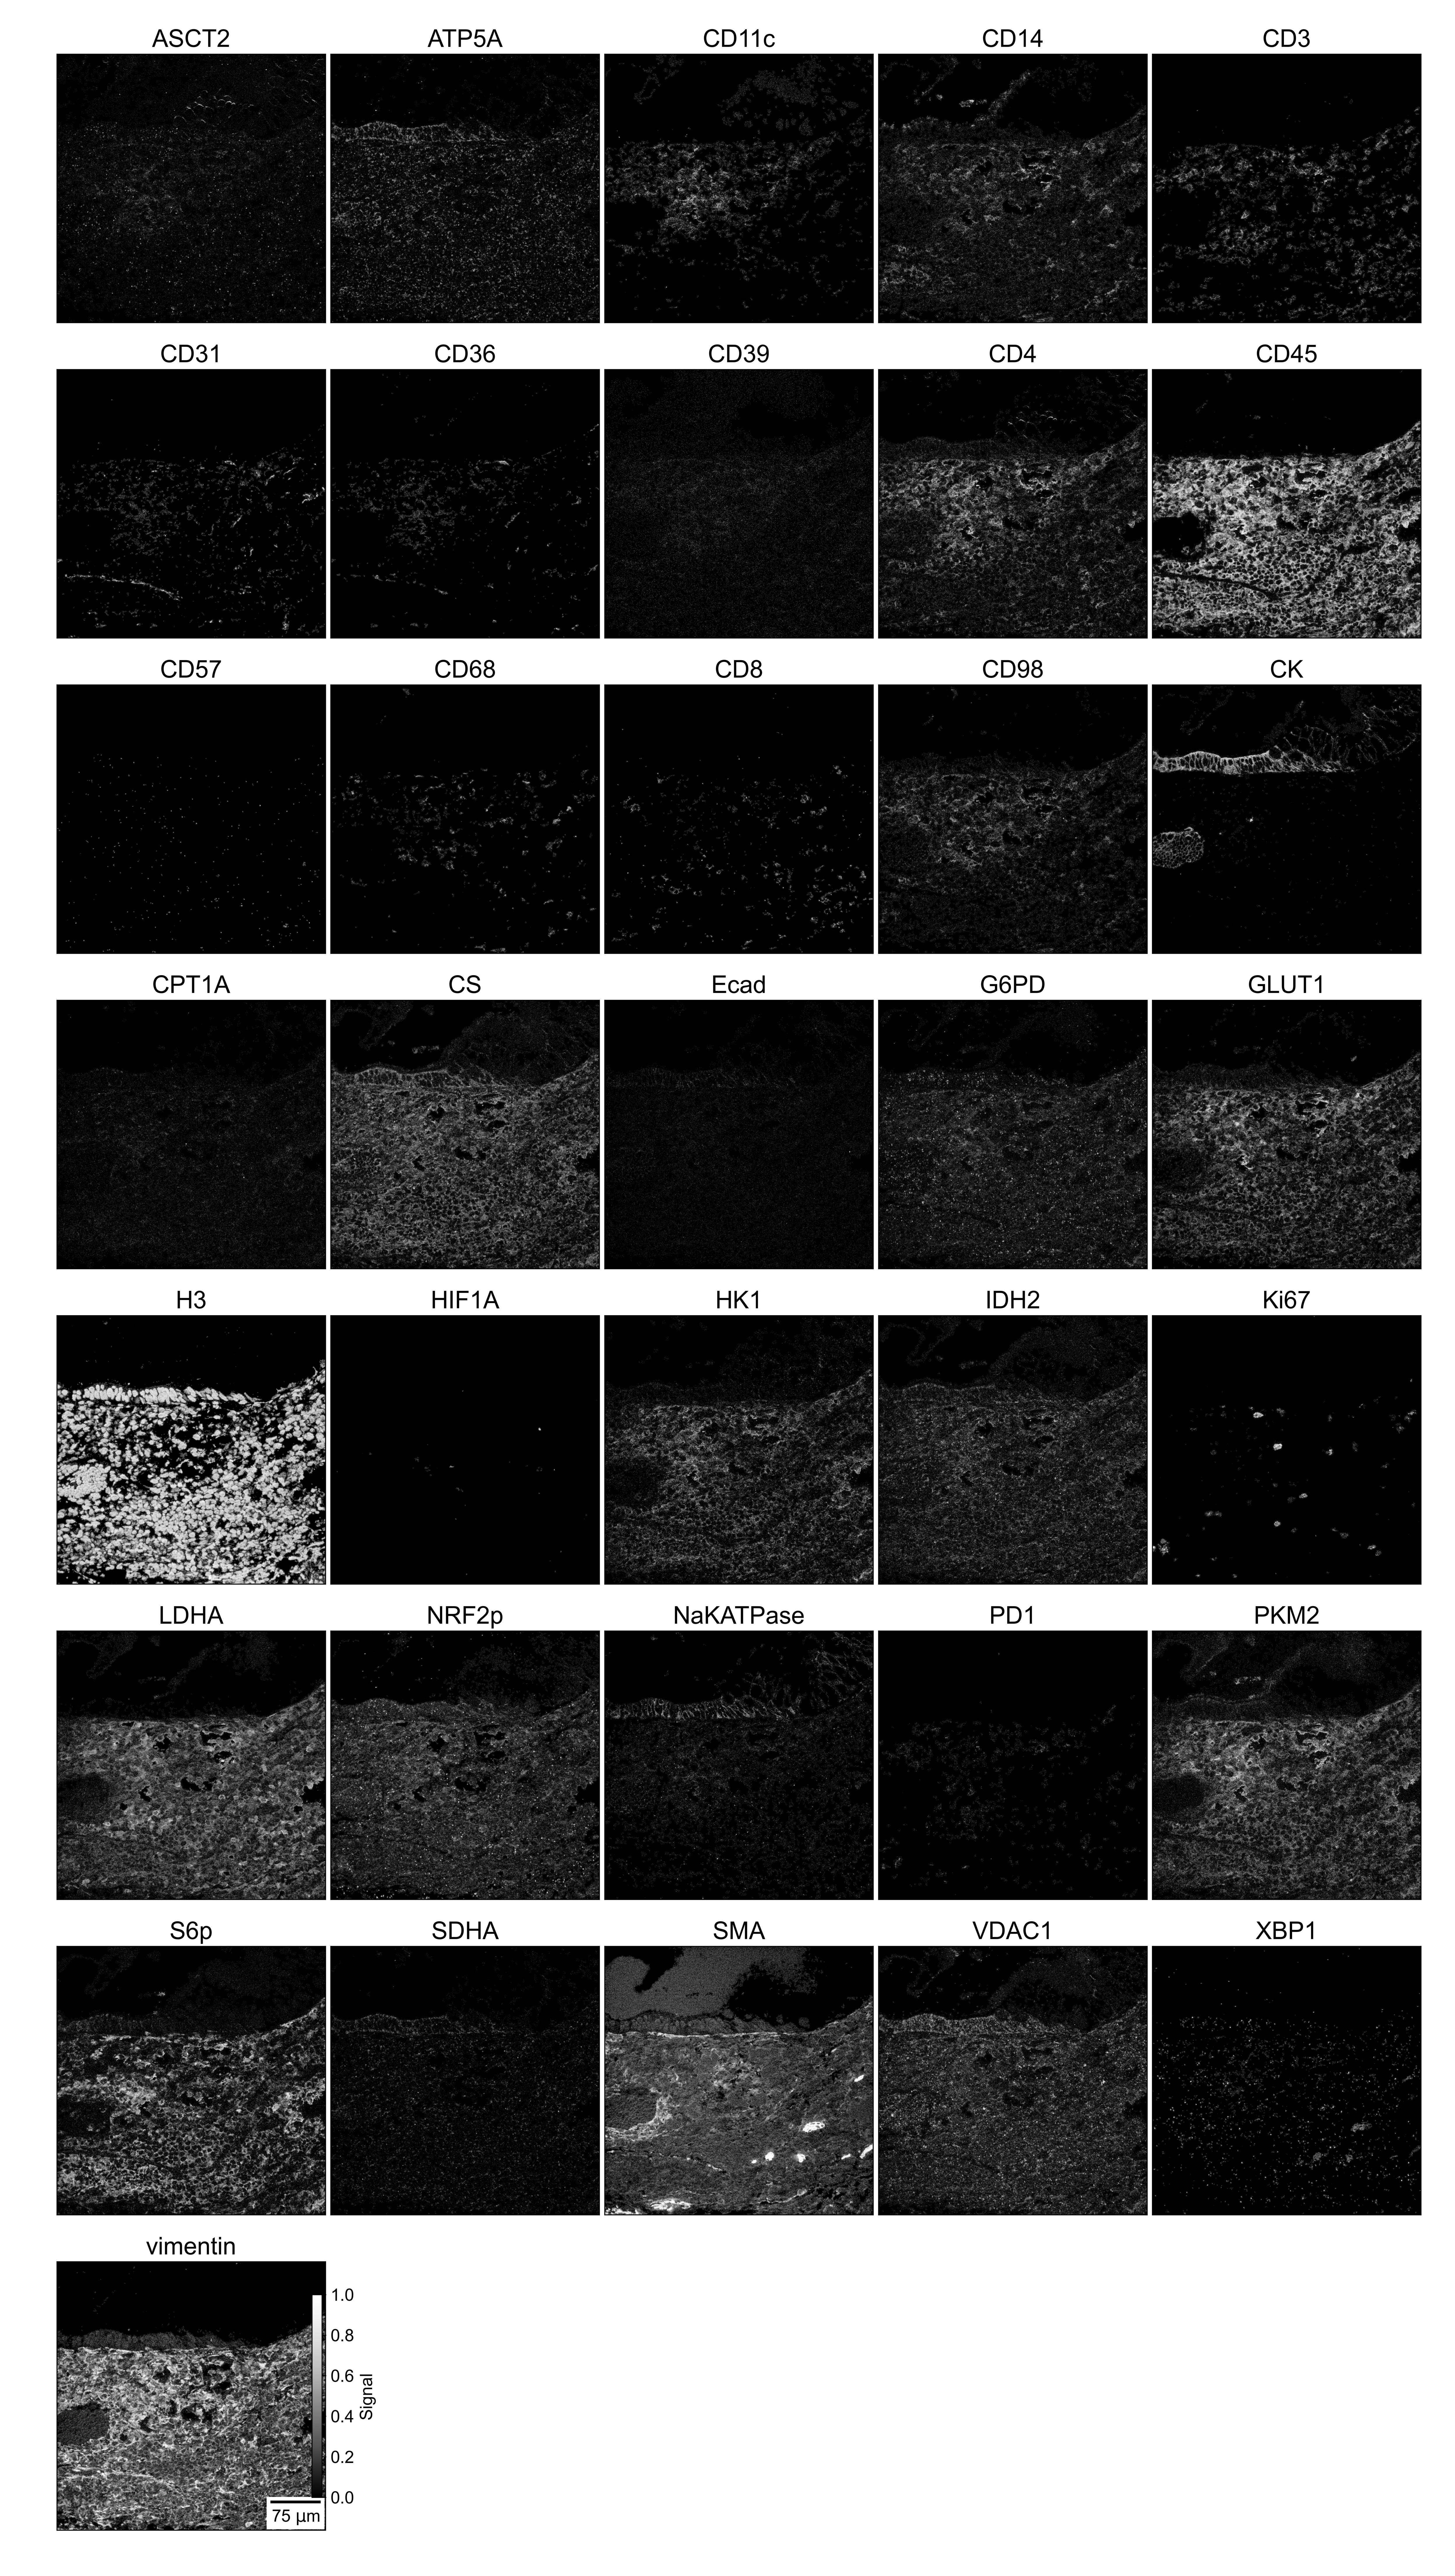
\includegraphics[width=14cm]{suppl-fig_healthy_sample_mibi_image}
    \caption{\textbf{MIBI-TOF image of the healthy colon sample "Point49".} Represented are the images of all 36 channels showing the signal of the respective proteins. The images were log1p transformed and represen the detected signal (metal-isotopes).}
    \label{fig:sup2}
\end{figure}

\pagebreak
